\documentclass[12pt, french]{article}
\usepackage{ae,lmodern}
\usepackage[french]{babel}
\usepackage[utf8]{inputenc}
\usepackage[T1]{fontenc}
\usepackage[dvipsnames]{xcolor}
\usepackage{graphicx}
\usepackage{hyphenat}
\usepackage[left=15mm, right=15mm]{geometry}
\geometry{
    a4paper,
    total={170mm,257mm},
    top=30mm,
 }
\usepackage{csquotes}
\usepackage{bookmark}
\usepackage{biblatex}
\usepackage{listings}
\usepackage{hyperref}
\usepackage{subcaption}
\usepackage{fancyhdr}

\hypersetup{
    hidelinks,
}
\usepackage{eurosym}

\addbibresource{rapport.bib}

\lstset{
  aboveskip=3mm,
  belowskip=-2mm,
  backgroundcolor=\color{lightgray},
  basicstyle=\footnotesize,
  breakatwhitespace=false,
  breaklines=true,
  captionpos=b,
  commentstyle=\color{ForestGreen},
  deletekeywords={\ldots},
  escapeinside={\%*}{*)},
  extendedchars=true,
  framexleftmargin=16pt,
  framextopmargin=3pt,
  framexbottommargin=6pt,
  frame=tb,
  keepspaces=true,
  keywordstyle=\color{blue},
  literate=
  {²}{{\textsuperscript{2}}}1
  {⁴}{{\textsuperscript{4}}}1
  {⁶}{{\textsuperscript{6}}}1
  {⁸}{{\textsuperscript{8}}}1
  {€}{{\euro{}}}1
  {é}{{\'{e}}}1
  {è}{{\`{e}}}1
  {ê}{{\^{e}}}1
  {ë}{{\¨{e}}}1
  {É}{{\'{E}}}1
  {Ê}{{\^{E}}}1
  {û}{{\^{u}}}1
  {ù}{{\`{u}}}1
  {â}{{\^{a}}}1
  {à}{{\`{a}}}1
  {á}{{\'{a}}}1
  {ã}{{\~{a}}}1
  {Á}{{\'{A}}}1
  {Â}{{\^{A}}}1
  {Ã}{{\~{A}}}1
  {ç}{{\c{c}}}1
  {Ç}{{\c{C}}}1
  {õ}{{\~{o}}}1
  {ó}{{\'{o}}}1
  {ô}{{\^{o}}}1
  {Õ}{{\~{O}}}1
  {Ó}{{\'{O}}}1
  {Ô}{{\^{O}}}1
  {î}{{\^{i}}}1
  {Î}{{\^{I}}}1
  {í}{{\'{i}}}1
  {Í}{{\~{Í}}}1,
  morekeywords={*,self, \_\_init\_\_, \_\_eq\_\_, \_\_str\_\_},
  numbers=left,
  numbersep=10pt,
  numberstyle=\tiny\color{black},
  rulecolor=\color{black},
  showspaces=false,
  showstringspaces=false,
  showtabs=false,
  stepnumber=1,
  stringstyle=\color{ForestGreen},
  tabsize=4,
  title=\lstname,
}

\title{
	\Huge
	\textbf{Application météo}
	\vspace{0.4cm}

	\LARGE
	Application Web et Sécurité
}

\author{
	Melissa Allaoua \\
    LE DENMAT Mickaël \\
    Hasnae Gaizi \\
    Gabriel Scrève \\
}

\begin{document}
	\begin{titlepage}
    \begin{center}
        \vspace*{1cm}

        \Huge
        \textbf{Application météo}

        \vspace{0.4cm}
        \LARGE
        Application Web et Sécurité

        \vspace{1.6cm}

        \large
        Melissa Allaoua \\
        Mickaël Le Denmat \\
        Hasnae Gaizi \\
        Gabriel Scrève \\

        \vspace{10cm}

        
\includegraphics[width=0.32\textwidth]{images/UVSQ-logo}

        \vspace{0.4cm}

        \Large
        Université de Versailles Saint-Quentin-en-Yvelines \\
        \vspace{0.4cm}
        15 Mai 2022
    \end{center}
\end{titlepage}
    \pagestyle{fancy} 
    \fancyhead[L]{Application Météo}
    \fancyhead[R]{\thepage}
    \fancyhead[C]{}
    \fancyfoot[C]{}
	\newpage
	\renewcommand{\contentsname}{Table des matières}
	\tableofcontents

	\newpage
	\section{Introduction}
	Consulter les prévisions météorologiques est devenu un réflexe quotidien pour de nombreuses personnes. Aujourd’hui, il existe une centaine d’applications différentes disponibles pour afficher la météo actuelle ainsi que les prévisions de la semaine au sein d’une disposition intelligente. Elles se mettent à jour à chaque changement de conditions climatiques et permettent aux utilisateurs de parcourir des plans de qualité d’air, de températures et différentes autres caractéristiques pour visualiser les différentes conditions climatiques dans une région.
	
	\section{Application météo}
		Notre projet est une application météo permettant à l'utilisateur d'afficher les informations météorologiques classiques en fonction de sa localisation, telles que
		la description de la météo du jour, la température,
		le ressenti, la vitesse du vent, etc. 
		Elle affiche également la température de la ville par tranche d'une heure ainsi que la météo du jour pour toute la semaine.
		
		\begin{figure}[htbp]
		    \centering
    		\begin{subfigure}{.7\textwidth}
    		    \centering
                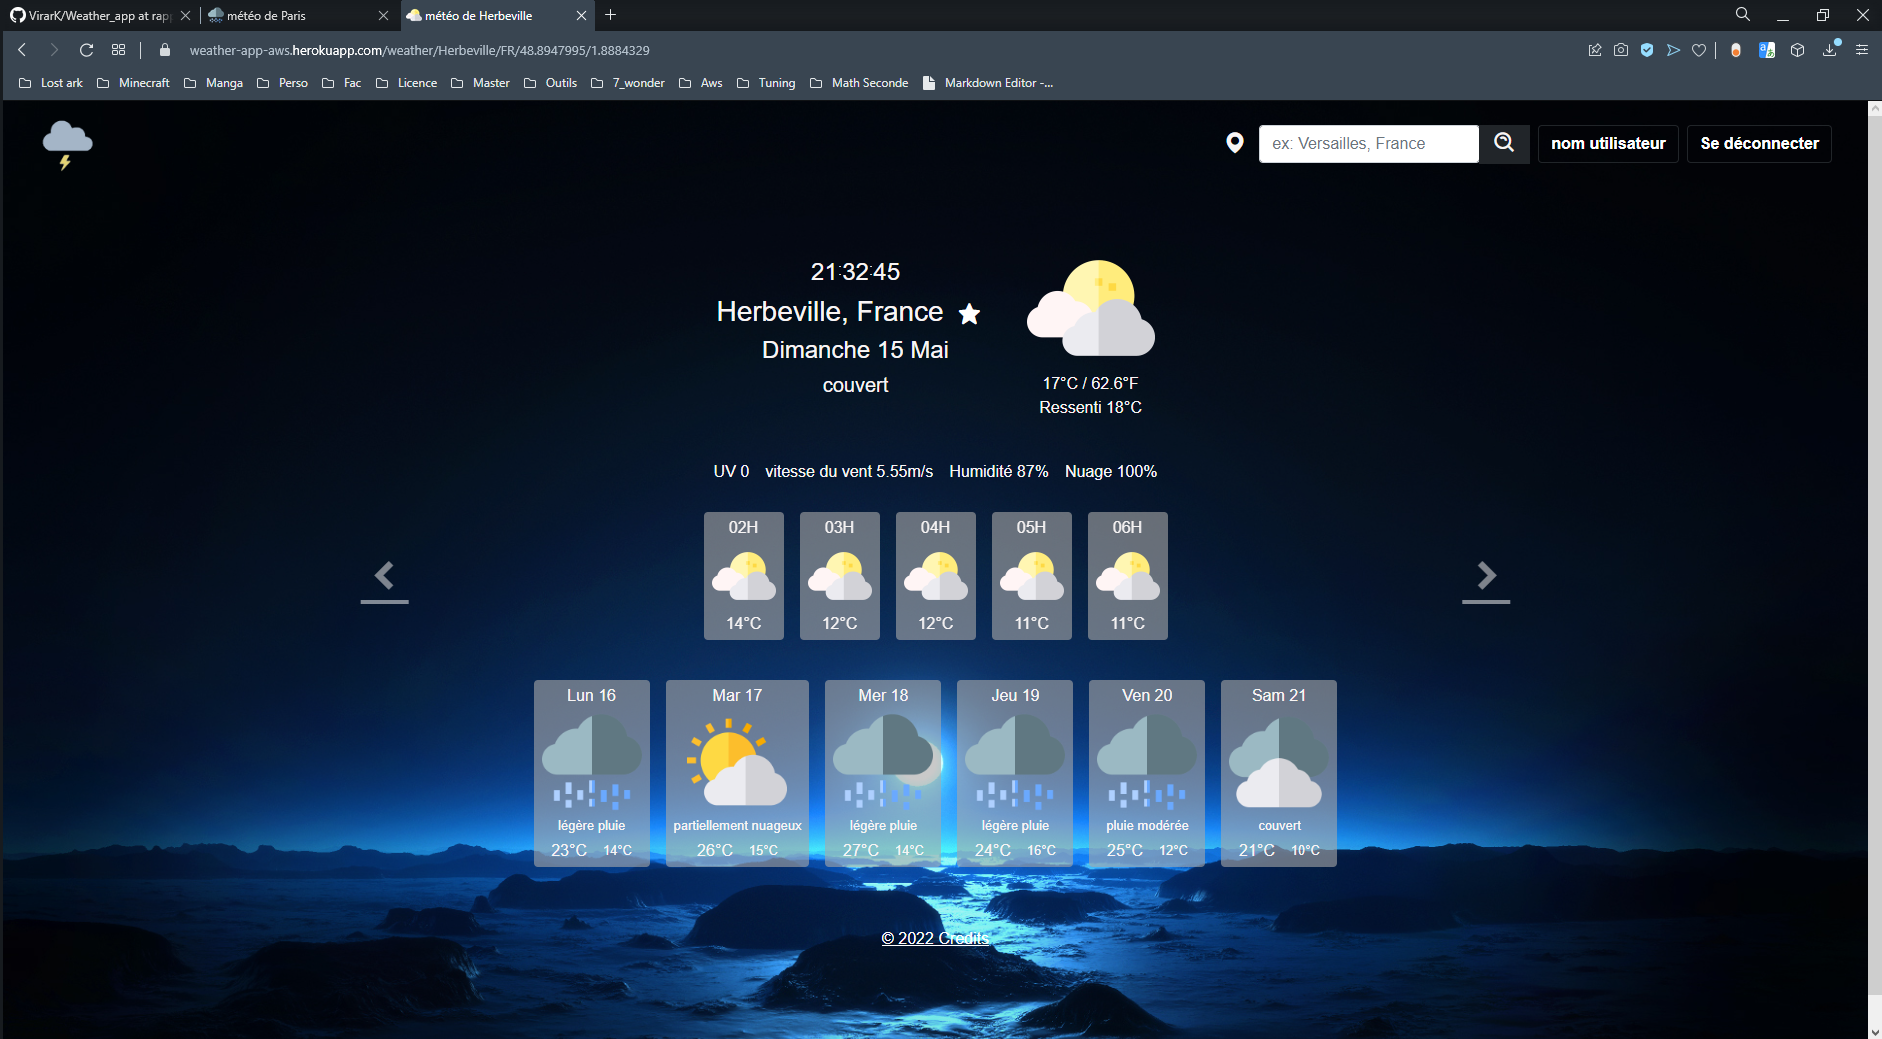
\includegraphics[width=\linewidth]{images/app_meteo.PNG}
                \caption{Application météo}
                \label{fig:Application_météo}
            \end{subfigure}
            \begin{subfigure}{.7\textwidth}
    		    \centering
                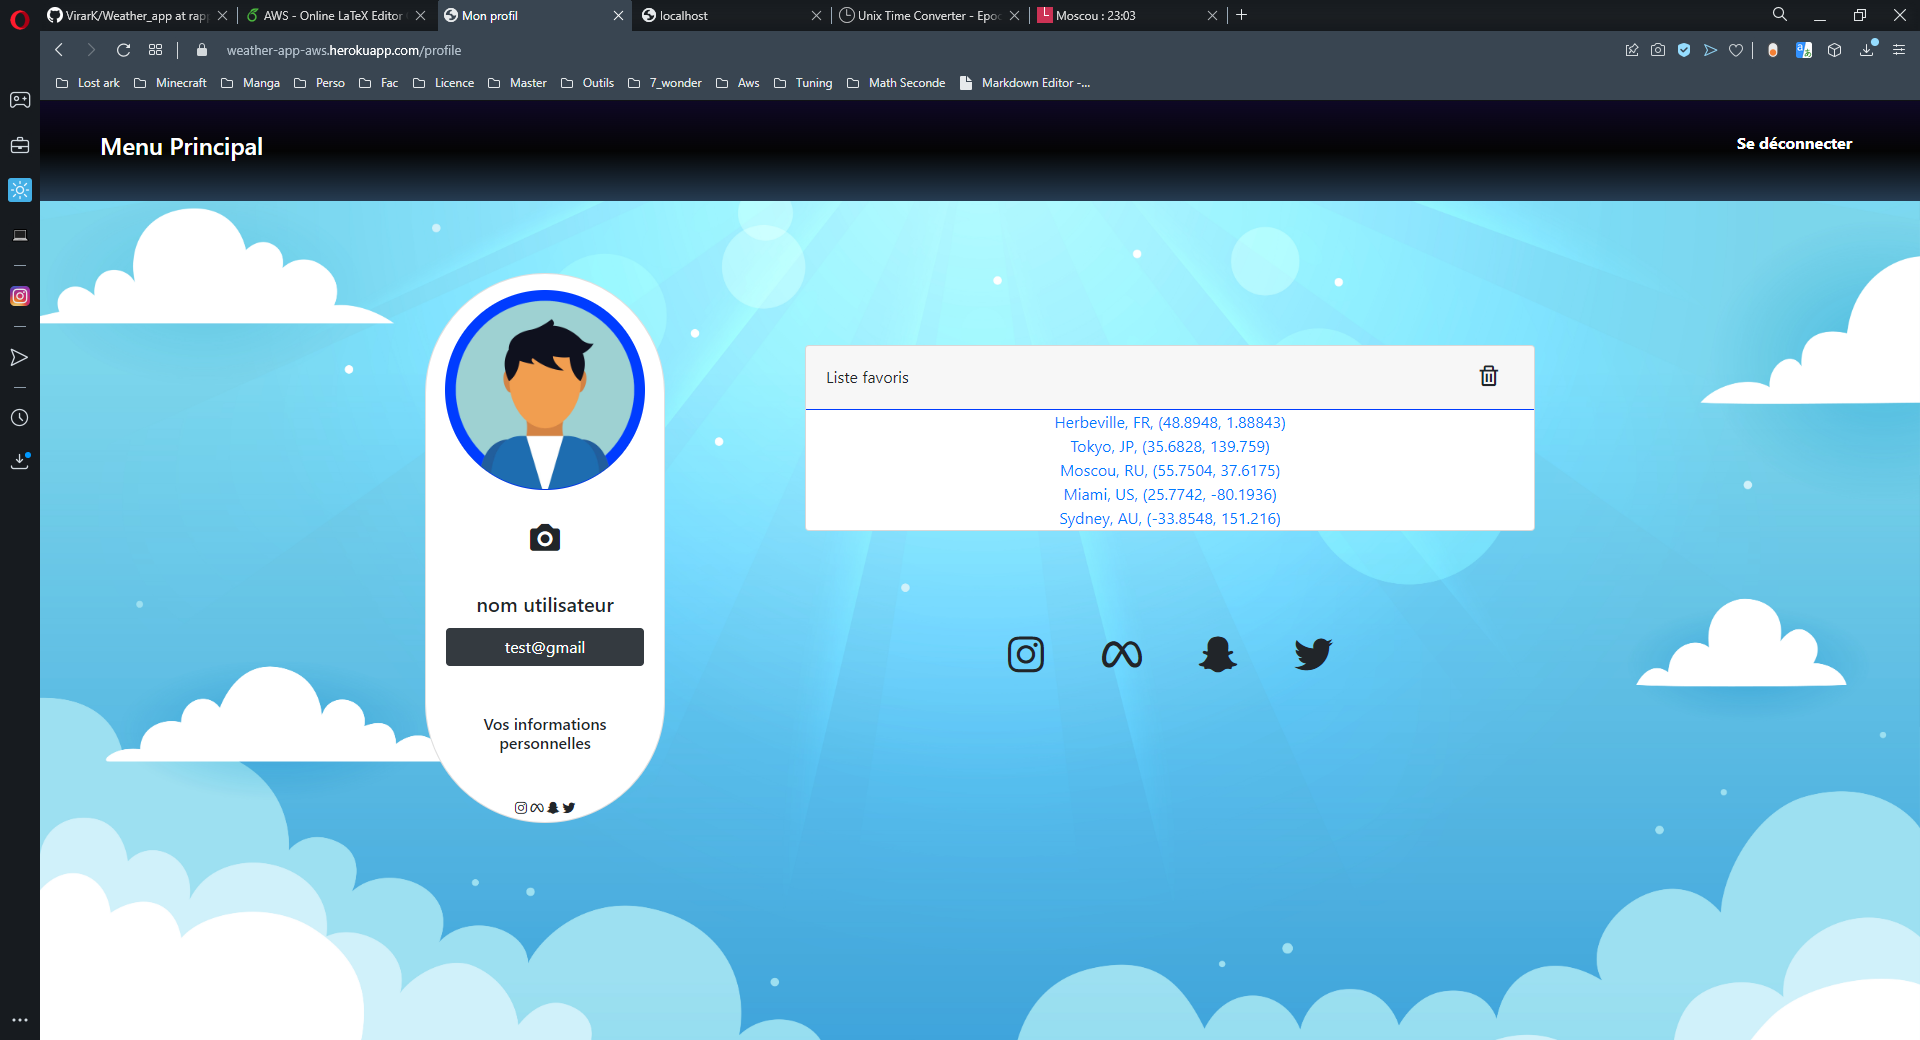
\includegraphics[width=\linewidth]{images/app_meteo_profile.PNG}
                \caption{Application météo}
                \label{fig:Application_météo}
            \end{subfigure}
            \caption{Application météo}
            \label{fig:Application_météo}
        \end{figure}
        
        \begin{center}
        L’utilisateur a la possibilité de créer un compte, de se connecter et d'ajouter des villes aux favoris afin de visualiser la météo de ses villes préférées plus facilement.
        \end{center}


	\section{Technologies utilisées}
		\subsection{Bootstrap}
			Bootstrap \cite{Bootstrap} est le framework HTML/CSS/JS le plus populaire pour le développement de sites dits \textit{responsive}. Utilisé pour construire des sites réactifs qui s'adaptent à toutes les tailles d'écrans ainsi que des sites pour les smartphones, nous l'avons choisi afin d'organiser les éléments au sein de notre application et  de la rendre réactive,
            c'est-à-dire découper les différentes pages en grilles et placer nos éléments où nous le souhaitons,
            utiliser les mises en forme de Bootstrap pour les boutons, les espaces entre les éléments, les couleurs, etc. \ Le site de Bootstrap propose aussi beaucoup de templates. \\ Nous avons en copié certains
			pour avoir une base fonctionnelle que nous avons modifiée pour
			ajouter ce dont nous avions besoin et pour que cela respecte le même
			style que notre application.\newline~~\\
			Beaucoup de frameworks existent mais Bootstrap présente plusieurs avantages : 
			\begin{itemize}
            \item[-]Tous les navigateurs modernes sont entièrement compatibles avec Bootstrap (Chrome, Firefox, Internet Explorer, Microsoft Edge, Safari et Opera),
            \item[-]Ses principaux styles de framework sont prédéfinis pour une approche \textit{mobile-first},
            \item[-]Il y'a beaucoup de  tutoriels Youtube ou autres et plus d'aide sur les forums en cas de bug,
            \item[-] Lors du developpement de l'application, Bootstrap a parfaitement collé à nos besoins, nous n'avons pas eu besoin de trouver une autre bibliothèque.
          \end{itemize}
        
          \textbf{Exemples de classes Bootsrap}
          \begin{itemize}
          \item[-].w-50 : l’élément a une largeur égale à 50\% de celle de son parent,
          \item[-] .h-100 : l’élément a une hauteur égale à celle de son parent,
          \item[-].h-auto : la hauteur de l’élément est définie automatiquement.
          \end{itemize}
          
		\subsection{Intégration de l'API}
		
		Il existe de nombreuses APIs météo, chacune avec un ensemble unique de fonctionnalités, des coûts variables et différents degrés de fiabilité. Certains ciblent même des marchés ou des communautés spécifiques avec des caractéristiques uniques pour les applications agricoles par exemple, ou encore la surveillance de la qualité de l'air. Avec les nombreuses options disponibles, choisir une API météo peut être un peu difficile.\newline~~\\
        \textbf{Choix de notre API:}~~\\
        Afin de choisir la meilleure API pour notre application, nous avons fait une comparaison des différentes APIs présentes en fonction des 4 points suivants :\newline
        \begin{itemize}
            \item[•] \textbf{fonctionnalités et portée :}~~\\
            Dans l'ensemble, la majorité des APIs  fournissent des données similaires, mais mais des éléments comme la durée de retour dans les enregistrements météorologiques historiques, ainsi que les formats de jour et d'heure varient.
            La plupart des APIs gratuites sont limitées non seulement par le nombre d'appels à ces dernières, mais également par les fonctionnalités fournies.\newline 
            \item[•] \textbf{Compatibilité et implémentation :}~~\\
            La plupart des APIs météo sont aujourd'hui basées sur l'architecture RESTful (une interface de programmation d'applications qui fait appel à des requêtes HTTP pour obtenir (GET), placer (PUT), publier (POST) et supprimer (DELETE) des données). Il faut prêter attention à ces différences subtiles dans les formats de date et d'heure, ainsi qu'à la compatibilité avec le framework de l'application et le langage utilisé.\newline
            Certaines APIs proposent une documentation, des tutoriels et des guides bien  approfondis, d'autres s'attendent à ce que l’utilisateur ait déjà une expérience antérieure dans la mise en œuvre d'APIs météo.\newline
            \item[•] \textbf{Réactivité et fiabilité :}
            La meilleure façon de savoir quelles APIs sont fiables et suffisamment rapides pour être intégrées à la version de production de l’application est de les essayer. Heureusement, la majorité d'entre elles proposent une option d'essai gratuite ou un abonnement freemium. Cela nous amène à une autre considération importante : le prix.\newline\\
            \item[•] \textbf{Coût :}
            Comme on peut s'y attendre, les fonctionnalités, la disponibilité, la capacité et la réactivité offertes par les services API gratuits sont inférieures à celles des options payantes.\newline
    
        \end{itemize}
            Le choix de l'API d'\textbf{OpenWeatherMap} \cite{OpenWeatherMap}  s’est basé principalement sur les fonctionnalités fournies dont nous avions le plus besoin pour la réalisation de  notre application ainsi que sur le nombre d’appels à l'API par jour dont on aura besoin.\newline~~\\
        \textbf{\underline{OpenWeatherMap:}}\newline
        
        	OpenWeatherMap est site proposant des services concernant la météo. Il permet
			de faire des requêtes à ses différentes APIs pour connaître la météo actuelle
			ou heure par heure, les prévisions de la semaine, l'humidité, l'indice UV, etc.\\
			Nous utilisons une de leurs APIs appelée \textit{OneCall} 
			qui nous permet d'obtenir toutes les informations essentielles en un seul appel.
			Grâce au JSON contenant la météo actuelle, nous récuperons des prévisions méteorologiques pour
			les heures à venir ainsi que pour toute la semaine.\newline~~\\
			L'appel à l'API se fait comme cela : \\
			\textit{https://api.openweathermap.org/data/2.5/onecall?lat={lat}\& \\
			lon={lon}\&appid={open\_weather\_key}\&lang=fr\&units=metric\&exclude=minutely,alerts}\newline~~\\
			Nous utilisons ensuite une variante de cette dernière afin d'avoir les informations
			concernant la météo des heures passées.\newline
			Pour cela nous faisons appel à:\\ 
			\textit{https://api.openweathermap.org/data/2.5/onecall/
			timemachine?lat={lat}\&lon={lon}\&dt={time}\&appid={API key}}.\newline\\
			Les deux appels à l'API fonctionnent avec différents paramètres :
			\begin{itemize}
			    \item[-]{\makebox[1.5cm]{$lat$\hfill}: la latitude de la ville,}
			    \item[-]{\makebox[1.5cm]{$lon$\hfill}: la longitude de la ville,}
			    \item[-]{\makebox[1.5cm]{$appid$\hfill}: la clé de l'API,}
			    \item[-]{\makebox[1.5cm]{$lang$\hfill}: la langue,}
			    \item[-]{\makebox[1.5cm]{$units$\hfill}: l'unité,}
			    \item[-]{\makebox[1.5cm]{$exclude$\hfill}: les informations qui ne nous intéressent pas et que nous excluons de la réponse,}
			    \item[-]{\makebox[1.5cm]{$dt$\hfill}: le "unix time", le nombre de secondes écoulées depuis le 1 Javnier 1970}
			\end{itemize}~~\\
			Grâce à ces deux APIs nous avons toutes les informations nécéssaires pour la réalisation notre projet.\newline
			
			L’appel à l’API nous a permis également de récupérer des informations concernant la date actuelle, le lever et le coucher du soleil (sunrise/sunset), ce qui nous a été utile pour l’implémentation des différentes fonctions de changement de l’affichage: changement des couleurs du texte ainsi que les images du fond en fonction de jour/nuit selon la ville recherchée.

		\subsection{Node js}
		Node.js \cite{NodeJS} est un environnement d’exécution single-thread, open-source permettant de créer des applications rapides côté serveur et en réseau. Il est non bloquant pour les entrées/sorties, ce qui permet d'avoir plusieurs clients faisant leurs demandes au serveur sans que le traitement de la demande de l'un bloque les autres, ce qui le rend efficace et adapté aux applications en temps réel. Il est souvent utilisé dans des applications de base de données avec MySQL. Il est aussi très simple à manipuler une fois que le javascript est maîtrisé.\\
		Nous l'utilisons pour créer un serveur en localhost afin d'hérberger notre application lors du développement. Une fois l'hébergement fait en ligne il nous sert à gérer la partie serveur.
		
		\subsection{MySQL}
		MySQL \cite{MySQL} est un système de gestion de base de données relationnelles open-source en SQL. Nous avons fait un schéma entité-relation (voir figure \ref{fig:entite_relation}) afin de voir les tables et les relations ainsi que des attributs dont nous avions besoin, puis nous avons créé les tables sur MySQL. Nous avons besoin de trois tables : deux entités et une relation.\newline
		\begin{figure}[htbp]
            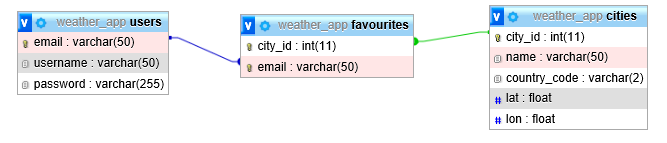
\includegraphics{images/schema_entite_relation.PNG}
            \caption{Schéma entité-relation}
            \label{fig:entite_relation}
        \end{figure}\newline~~\\
        
		\textbf{La table users} nous permet de stocker les utilisateurs, représenté par un email (clé primaire), un username, et un mot de passe (ce dernier est hashé pour des raisons de sécurité mais nous en parlerons plus tard).\newline 
		
	    \textbf{La table cities} représentant une ville avec un numéro de ville qui s'incrémente à chaque ajout (clé primaire), un nom, un code de pays, une latitude et une longitude.\newline
	    
		\textbf{La table favourites} qui représente l'association entre un utilisateur et la ville qu'il ajoute en favoris. Elle contient les clés primaires des deux tables.
		
		\begin{figure}[htbp]
		    \centering
    		\begin{subfigure}{.4\textwidth}
                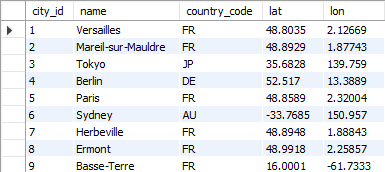
\includegraphics[width=\linewidth]{images/cities.PNG}
                \caption{Table "cities"}    
    		\end{subfigure}
    		\hfill
            \begin{subfigure}{.35\textwidth}
                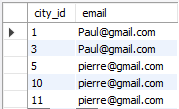
\includegraphics[width=.8\linewidth]{images/favourites.PNG}
                \caption{Table "favourites"}
            \end{subfigure}
            \hfill
            \begin{subfigure}{.45\textwidth}
                \hspace{-2.5cm}.
                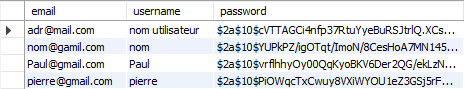
\includegraphics[width=1.5\linewidth]{images/users.PNG}
                \caption{Table "users"} 
            \end{subfigure}
            \caption{Exemple d'entrées dans la base de données}
        \end{figure}
		
		\newpage
		\subsection{Express JS}
		Express \cite{ExpressJS} est un framework très utilisé de Node.js car comme Node.js est simple à utiliser, une fois le javascript maîtrisé, il est assez complet et très perfomant pour un premier projet avec du backend. Il a pour objectif de gérer les requêtes et les réponses entre le client et le serveur, de traiter les sessions des utilisateurs et de faire le routages. \\
		Il nous a permit de créer les différentes routes du projet, en commençant par \textbf{l'index "/"}, la route pour la météo \textbf{"/weather"} complété par le chemin \textbf{"/:city/:country\_code/:lat/:lon"} afin d'afficher la météo et la route \textbf{"/profile"} pour la page de profile de l'utilisateur. Puis la route \textbf{"/auth"} pour le système de connection et de déconnexion (\textbf{"/auth/login"} pour la connection, \textbf{"/auth/register"} pour l'inscription et \textbf{"/auth/logout"} pour la déconnexion). Et enfin la route \textbf{"/favourites"} pour les favoris (\textbf{"/favourites/new/:city/:country\_code/:lat/:lon"} pour ajouter, \textbf{"/favourites/new/:city/:country\_code/:lat/:lon"} pour supprimer et \textbf{"/favourites/clear"} pour supprimer tous les favoris).
		
		\subsection{Handlebars}
		Handlebars\cite{Handlebars} est un modèle proche de HTML mais en y ajoutant des éléments de logique issue de la programmation comme les boucles (for,...), les conditions (if, else if, ...) et d'autres fonctionnalités. \\
		Il nous a permis d'ajouter des conditions afin de modifier l'affichage d'une page en fonction de la valeur de retour d'une fonction comme dans cet exemple :\newpage
		% NE PAS TABULER LE CODE
		\begin{lstlisting}[language=html]
{{#if user}}
	{{#if is_favourite}}
		<button
			onclick="del_favourite()"
			class="btn btn-outline favoris"
			title="Cliquez pour supprimer des favoris"
		>
		<i class="bx bxs-star bx-sm" style="color: rgb(231, 185, 85)">
		</i>
		</button>
	{{else}}
		<button
			onclick="new_favourite()"
			class="btn btn-outline favoris"
			title="Cliquez pour ajouter au favoris"
		>
		<i class="bx bxs-star bx-sm" style="color: rgb(255, 255, 255)">
		</i>
		</button>
	{{/if}}
{{/if}}\end{lstlisting}
		
		Si l'utilisateur est connecté et si la ville est en favoris alors nous affichons une étoile jaune, mais si elle n'est pas en favoris alors nous affichons une etoile blanche.
		
		\begin{figure}[htbp]
    		\begin{subfigure}{.33\textwidth}
		        \centering
                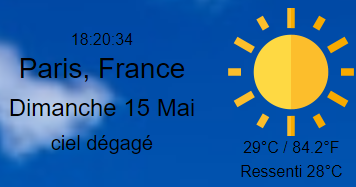
\includegraphics[width=.82\linewidth]{images/user_non_connecte.PNG}
                \caption{Utilisateur non connecté}
                \label{fig:user_non_connecte}      
    		\end{subfigure}
            \begin{subfigure}{.33\textwidth}
                \centering
                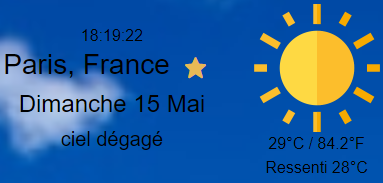
\includegraphics[width=.9\linewidth]{images/user_connecte_fav.PNG}
                \caption{Ville en favoris}
                \label{fig:user_connecte_fav}   
            \end{subfigure}
            \begin{subfigure}{.33\textwidth}
                \centering
                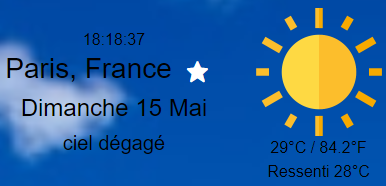
\includegraphics[width=.9\linewidth]{images/user_connecte_non_fav.PNG}
                \caption{Ville pas en favoris}
                \label{fig:user_connecte_non_fav}
            \end{subfigure}
            \caption{Différence d'affichage avec Handlebars}
        \end{figure}
        
        {\parindent0pt
            Nous l'avons aussi utilisé pour afficher des erreurs lors du remplissage du formulaire d'inscription. Enfin, nous l'avons aussi utilisé afin d'ajouter des boucles pour parcourir tous les favoris de l'utilisateur et les afficher dans sa page de profil comme dans cette exemple :
    		
    		% NE PAS TABULER LE CODE
		    \begin{lstlisting}[language=html]
{{#if favs}}
    {{#each favs}}
          <div><a href="/weather/{{this.name}}/{{this.country_code}}/{{this.lat}}/{{this.lon}}">{{this.name}}, {{this.country_code}}, ({{this.lat}}, {{this.lon}})</a></div>
    {{/each}}
{{else}}
    <div>Aucun favori !</div>
{{/if}}
		    \end{lstlisting}
        }
		\newpage
		\subsection{Bcrypt}
		Bcrypt\cite{Bcrypt} est un algorithme de hashage qui nous sert à encoder les mots de passe afin de sécuriser les données des utilisateurs. Nous avons intégré cet algorithme à notre site en utilisant la librairie NodeJS proposée. Chaque mot de passe utilisé lors de la création d'un compte est hashé avec bcrypt avant d'être envoyé à la base de données. Un grain de sel est utilisé afin de sécuriser le hash produit. Lorsqu'un utilisateur veut se connecter, on compare le hash du mot de passe qu'il a entré avec celui présent sur la base de données.
		\begin{center}
		\begin{figure}[!h]
		    \centering
		    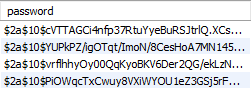
\includegraphics[width=.51\linewidth]{images/mdp.png}
		    \caption{Mots de passe stockés dans la base de données}
		    \label{fig:mdp}
		\end{figure}
		    
		\end{center}
		
		\subsection{JWT}
		    JWT\cite{JWT}, pour JSON Web Token, est un jeton d'accès stockant toutes les informations nécéssaires afin de nous permettre d'identifier l'utilisateur de l'application. 
		    Nous stockons dans ce token l'email de l'utilisateur, la date de création du token ainsi que sa date d'expiration. Ce token est signé avec un secret stocké sur notre hébergeur, Heroku. Le secret permet d'authentifier le token, afin qu'il puisse être utilisé pour le maintien de la connexion. Ce token est lui-même stocké en tant que cookie, et le cookie est supprimé dès qu'un utilisateur se déconnecte ou que la date d'expiration est dépassée.

		\subsection{Hébergement du site}
		    Pour héberger le site, nous avons choisi d'utiliser Heroku\cite{Heroku}.
		    Heroku est une plateforme en tant que service basée sur le cloud (PaaS) qui a été conçue par des développeurs pour les développeurs.
		    Cette solution aide les développeurs et les entreprises à créer et faire évoluer leurs applications de la meilleure façon possible.\\
		    \textbf{Quelques caractèristiques de Heroku}
		     \begin{itemize} 
		     \item[-]\textbf{Runtime Heroku :}
		     Cette plateforme exécute les applications dans des conteneurs intelligents et fiables appelés dynos.
		     \item[-]\textbf{Service de données et écosystème :}
		     Heroku offre une disponibilité et un basculement automatique avec son service de base de données hébergé.
             \item[-]\textbf{Sécurité et conformité :}
             Offre la possibilité de stocker les applications sensibles sur Heroku en raison des normes de sécurité de haut niveau.
		     \end{itemize}~~
            Nous utilisons la version gratuite d'Heroku, à laquelle nous avons ajouté un add-on intégré à Heroku pour le stockage de base de données, JawsDB \cite{JawsDB}.\newline
            
        \textit{\textbf{Le site de notre application météo:}} \url{https://weather-app-aws.herokuapp.com/}. 
	
	\newpage
	\section{Quelques bugs et améliorations à apporter}
	Notre projet est plutôt complet en général, il regroupe les fonctionnalités que nous avions dans nos objectifs initiaux. Cependant, afin de pouvoir concurrencer les autres applications météo du marché, il existe beaucoup de fonctionnalités que nous pouvons ajouter :
    \begin{itemize}
        \item La possibilité pour l'utilisateur de modifier son profil (changer le mot de passe, son image de profil, son email, ou son nom),
        \item L'affichage général de notre application (faire des fonds personnalisés au lieu de prendre ceux de notre API),
        \item Rendre notre site \textit{responsive} pour qu'il s'affiche correctement sur tous les appareils,
        \item Ajouter une fonction de récupération de mot de passe oublié,
        \item Ajouter des informations supplémentaires sur les conditions climatiques (carte de pollution de l'air, risques de tempêtes dans la zone, la pression de l'air, le risque de neige ou de verglas, ...),
        \item Permettre à l'utilisateur d'avoir plus de données sur le jour de la semaine souhaité
    \end{itemize}
    Pour les bugs de notre application, nous avons essayé de les réparer dès que nous en trouvions un. Un bug majeur est le fait que nous ne puissions pas encore stocker la photo que l'utilisateur a choisi de mettre sur son profil hors de sa session (il se connecte, modifie sa photo, mais si il se déconnecte, il perd sa photo). Un autre problème majeur est que si un utilisateur oublie son mot de passe, on ne peut pas lui retrouver et il doit recréer un compte.

	
	\section{Organisation du travail}
	Pour l'organisation de notre projet, il nous a fallu deux choses, premièrement un outil pour garder des traces de l'evolution du projet afin que tous les membres puissent y accéder et suivre son avancement, deuxièment un moyen de communication écrit et oral pour partager des liens, demander de l'aide, faire nos réunions (tous les dimanches en fin d'après-midi et tous les mercredis soir avant la présentation) et d'autres fois en cas de besoin. \\
	Pour le premier nous avons choisi GitHub, chacun des membres connaissant déjà l'outil et le maîtrise. Il nous permet un suivi du projet au cours des différentes modifications avec l'historique des commits et nous permet de faire des branches afin de développer des nouvelles fonctionnalités.\\
	Pour le deuxième, nous avons choisi Discord, chacun des membres l'utilisait et il offre beaucoup de services qui nous ont été grandement utiles comme par exemple la création différents channels pour retrouver le plus rapidement possible une information dite par un membre ou un lien, la création des channels vocaux pour faire nos réunions, partager nos écrans pour travailler ensemble ou aider un membre à débugger, etc.

	\section{Structure}
	Notre application est découpée en différents dossiers et sous-dossiers :
	\begin{itemize}
	    \item \texttt{controllers} qui contient tous les fichiers faisant des actions sensibles comme les requêtes à la base de données, les comparaisons avec bcrypt,...
	    \item \texttt{public} qui contient toutes les images affichées sur le site ainsi que les scripts de météo et les fichiers de style,
	    \item \texttt{routes} qui contient les scripts liés aux routes, 
	    \item \texttt{views} qui contient tous les fichiers \textit{.hbs},
	    \item \texttt{root} qui contient le fichier app.js ainsi que le fichier package.json.
	\end{itemize}
	\newpage
	\begin{figure}[!h]
	    \centering
	    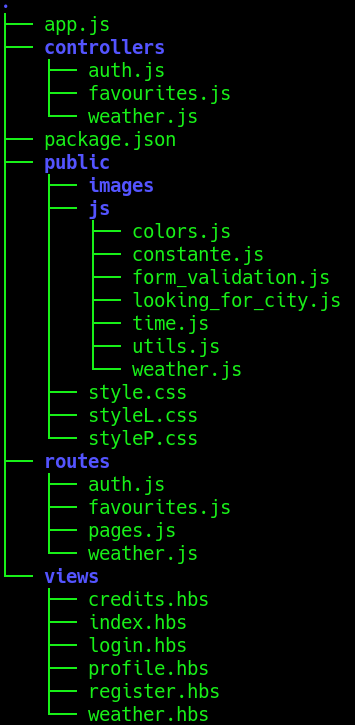
\includegraphics[width=.3\linewidth]{images/tree.png}
	    \caption{Structure de notre application}
	    \label{fig:tree}
	\end{figure}
	\newpage
	\section{Sources}
% 	\begin{itemize}
    \item \url{https://www.youtube.com/watch?v=VavWEtI5T7c&list=PLD9SRxG6ST3GBsczn8OUKLaErhrvOz9zQ} Tutoriel Nodejs et MySQL.
    \item \url{https://www.youtube.com/watch?v=dinW2QTSNl4} Tutoriel Expression regulière
    \item \url{https://www.esparkinfo.com/blog/node-js-with-mysql-using-sequelize-express.html} Tutoriel Node.js et MySQl.
    \item \url{https://www.youtube.com/watch?v=Zcg71lxW-Yo} Tutoriel Deploy MySQL Database to Heroku with ClearDB MySQL Add-on.
    \item \url{https://www.geeketfier.fr/archives/mots-de-passe-hashage-et-salage-suffisant/} Mots de passe : hashage et salage, suffisant ?
    \item \url{https://www.bcrypt.fr/questions} Questions Bcrypt.
    \item \url{https://momentjs.com/timezone/} Moment js Timezone.
    \item \url{https://github.com/moment/moment-timezone/blob/develop/data/packed/latest.json}.
    \item \url{https://latex-tutorial.com/tutorials/bibtex/} Bibliography in LaTeX with Bibtex/Biblatex.
    \item \url{https://www.eng.auburn.edu/~reevesj/Classes/ELEC6970-latex/Graphics/Graphics_in_LaTeX.pdf} Graphics in LATEX.
    \item \url{https://www.tomorrow.io/blog/top-8-weather-apis-for-2022/} Comparaison des APIs météo.
    \item \url{https://www.flaticon.com/free-icons/weather} Icônes en libres droits.
    \item \url{https://www.youtube.com/watch?v=5JHqEMGkHXY} Tutoriel application météo web.
    \item \url{https://www.iban.com/country-codes} Codes ISO internationaux.
    \item \url{https://unixtimeconverter.net} unixtimeconverter.
    \item \url{https://www.wampserver.com} wampserver.
    \item \url{https://www.w3schools.com/cssref/pr_background-image.asp}.
    \item \url{https://www.w3schools.com/bootstrap4/bootstrap_carousel.asp}.
    \item \url{https://stackoverflow.com/questions/8420740/url-not-defined};
    \item \url{https://bootstrapcreative.com/pattern/change-bootstrap-carousel-navigation-icons/}.
    \item \url{https://getbootstrap.com/docs/4.0/components/carousel/}.
    \item \url{https://getbootstrap.com/docs/4.0/utilities/flex/}.
    \item \url{https://getbootstrap.com/docs/5.0/utilities/text/}.
    \item \url{https://www.webfx.com/blog/web-design/responsive-background-image/}.
    \item \url{https://tex.stackexchange.com/questions/170316/nocite-for-single-bibdatasources-with-biblatex-biber}.
    \item \url{https://latex.org/forum/viewtopic.php?t=4580}.
    \item \url{https://masteringjs.io/tutorials/fundamentals/compare-strings-ignore-case}.
    \item \url{https://developer.mozilla.org/fr/docs/Web/JavaScript/Reference/Global_Objects/String/length}.
    \item \url{https://developer.mozilla.org/fr/docs/Web/JavaScript/Reference/Global_Objects/String/slice}.
    \item \url{https://www.geeksforgeeks.org/moment-js-moment-hour-method/}.
    \item \url{https://stackoverflow.com/questions/58912812/get-hours-minutes-seconds-from-moment-js-object}.
    \item \url{https://time.is/fr/Miami}.
    \item \url{https://cdnjs.com/libraries/moment.js}.
    \item \url{https://cdnjs.com/libraries/moment-timezone}.
    \item \url{https://stackoverflow.com/questions/15141762/how-to-initialize-a-javascript-date-to-a-particular-time-zone/15171030#15171030}.
    \item \url{https://stackoverflow.com/questions/10883441/clock-in-different-time-zones}.
    \item \url{https://www.youtube.com/watch?v=dbfyW99VTKo}.
    \item \url{https://stackoverflow.com/questions/10967736/how-to-use-moment-js}.
    \item \url{https://zetcode.com/javascript/momentjs/}.
    \item \url{https://stackoverflow.com/questions/37398871/javascript-get-current-date-using-utc-offset}.
    \item \url{https://www.geeksforgeeks.org/javascript-date-now-method/}.
    \item \url{https://stackoverflow.com/questions/19581683/get-value-of-div-content-using-jquery}.
    \item \url{https://www.w3schools.com/jquery/jquery_dom_get.asp}.
    \item \url{https://developer.mozilla.org/en-US/docs/Web/JavaScript/Reference/Global_Objects/Date/now}.
    \item \url{https://stackoverflow.com/questions/8647216/get-content-of-a-div-using-javascript}.
    \item \url{https://stackoverflow.com/questions/48200098/get-content-of-an-html-com-object-in-powershell}.
    \item \url{https://www.freecodecamp.org/news/javascript-date-now-how-to-get-the-current-date-in-javascript/}.
    \item \url{https://www.w3schools.com/jsref/jsref_now.asp}.
    \item \url{https://developer.mozilla.org/fr/docs/Web/JavaScript/Reference/Global_Objects/Date}.
    \item \url{https://www.w3schools.com/howto/howto_js_countdown.asp}.
    \item \url{https://bobbyhadz.com/blog/javascript-get-response-status-code-fetch}.
    \item \url{https://latex-tutorial.com/subfigure-latex/}.
    \item \url{https://stackoverflow.com/questions/36800861/moment-timezone-converting-a-date-to-unix}.
\end{itemize}
    \begin{itemize}
    \item \url{https://www.youtube.com/watch?v=VavWEtI5T7c&list=PLD9SRxG6ST3GBsczn8OUKLaErhrvOz9zQ} Tutoriel Nodejs et MySQL.
    \item \url{https://www.youtube.com/watch?v=dinW2QTSNl4} Tutoriel Expression regulière
    \item \url{https://www.esparkinfo.com/blog/node-js-with-mysql-using-sequelize-express.html} Tutoriel Node.js et MySQl.
    \item \url{https://www.youtube.com/watch?v=Zcg71lxW-Yo} Tutoriel Deploy MySQL Database to Heroku with ClearDB MySQL Add-on.
    \item \url{https://www.geeketfier.fr/archives/mots-de-passe-hashage-et-salage-suffisant/} Mots de passe : hashage et salage, suffisant ?
    \item \url{https://www.bcrypt.fr/questions} Questions Bcrypt.
    \item \url{https://momentjs.com/timezone/} Moment js Timezone.
    \item \url{https://github.com/moment/moment-timezone/blob/develop/data/packed/latest.json}.
    \item \url{https://latex-tutorial.com/tutorials/bibtex/} Bibliography in LaTeX with Bibtex/Biblatex.
    \item \url{https://www.eng.auburn.edu/~reevesj/Classes/ELEC6970-latex/Graphics/Graphics_in_LaTeX.pdf} Graphics in LATEX.
    \item \url{https://www.tomorrow.io/blog/top-8-weather-apis-for-2022/} Comparaison des APIs météo.
    \item \url{https://www.flaticon.com/free-icons/weather} Icônes en libres droits.
    \item \url{https://www.youtube.com/watch?v=5JHqEMGkHXY} Tutoriel application météo web.
    \item \url{https://www.iban.com/country-codes} Codes ISO internationaux.
    \item \url{https://unixtimeconverter.net} unixtimeconverter.
    \item \url{https://www.wampserver.com} wampserver.
    \item \url{https://www.w3schools.com/cssref/pr_background-image.asp}.
    \item \url{https://www.w3schools.com/bootstrap4/bootstrap_carousel.asp}.
    \item \url{https://stackoverflow.com/questions/8420740/url-not-defined};
    \item \url{https://bootstrapcreative.com/pattern/change-bootstrap-carousel-navigation-icons/}.
    \item \url{https://getbootstrap.com/docs/4.0/components/carousel/}.
    \item \url{https://getbootstrap.com/docs/4.0/utilities/flex/}.
    \item \url{https://getbootstrap.com/docs/5.0/utilities/text/}.
    \item \url{https://www.webfx.com/blog/web-design/responsive-background-image/}.
    \item \url{https://latex.org/forum/viewtopic.php?t=4580}.
    \item \url{https://masteringjs.io/tutorials/fundamentals/compare-strings-ignore-case}.
    \item \url{https://developer.mozilla.org/fr/docs/Web/JavaScript/Reference/Global_Objects/String/length}.
    \newpage
	\printbibliography
\end{itemize}
\end{document}
